\documentclass{beamer}

%\usepackage{beamerthemetreebars}
\usepackage{graphicx}
%\usepackage{beamerthemesplit}
%\beamertemplateshadingbackground{red!10}{blue!10}

%----------------------------------------------------------------------
% Para que aparezcan varias transparencias en la misma p\'{a}gina
\usepackage{pgfpages}
%\pgfpagesuselayout{4 on 1}[a4paper,border shrink=5mm,landscape]
%----------------------------------------------------------------------
% Suprime los s\'{\i}mbolos de navegaci\'{o}n
\setbeamertemplate{navigation symbols}{}
%---------------------------------------------------------------------

\usepackage[utf8]{inputenc}
%----------------------------------------------------------------
\newcommand{\ep}{\epsilon}
\newcommand{\real}{{\rm I\kern-.17em R}}
\newcommand{\pro}{\mbox{P}}
%-----------------------------------------------------------------

\title[Estad\'{\i}stica: Tema 1]{Tema 1\\
 Introducción}
\author[Berrendero]
{Jos\'{e} R. Berrendero}
\date{}
\institute{Departamento de Matem\'{a}ticas\\
 Universidad Aut\'{o}noma de Madrid}

%------------------------------------------------------------

\begin{document}

\frame{\titlepage}
%\section[Outline]{}
%\frame{\tableofcontents}

%------------------------------------------------------------------
% Aqu\'{\i} empieza la presentaci\'{o}n
%------------------------------------------------------------------

\begin{frame}[plain]
\frametitle{Informaci\'{o}n de contacto}


\centerline{Jos\'{e} Ram\'{o}n
Berrendero D\'{\i}az}

\bigskip

\bigskip

\textbf{Correo electr\'{o}nico:} {\tt joser.berrendero@uam.es}

\bigskip

\textbf{Tel\'{e}fono:} 91 497 66 90

\bigskip

\textbf{Despacho:}  M\'{o}dulo 08 - Despacho 210

\bigskip

\textbf{P\'{a}gina web:} {\tt http://www.uam.es/joser.berrendero}

%(Hay un enlace a la asignatura) %{\em An\'{a}lisis de datos}


\end{frame}
%----------------------------------------------------------------------


%-------------------------------------------------------------------------
\begin{frame}[plain]
\frametitle{Temario}

\begin{enumerate}

\item Introducción.


\

\item Conjuntos convexos.

\



\item Optimización lineal. El algoritmo del simplex.



\


\item Funciones convexas y optimización convexa.

\

\item  Dualidad y condiciones de Karush-Kuhn-Tucker.

\

\item Aplicaciones.



\end{enumerate}



\end{frame}
%----------------------------------------------------------------------
\begin{frame}[plain]
\frametitle{Bibliograf\'{\i}a básica}

\begin{itemize}



\item Bazaraa, M. S., Jarvis, J. J. y Sherali, H. D. (2011). \textit{Linear programming and network flows}. John Wiley \& Sons.

\

\item Bazaraa, M. S., Sherali, H. D. y Shetty, C. M. (2013). \textit{Nonlinear programming: theory and algorithms}. John Wiley \& Sons.

\

\item Boyd, S. y Vandenberghe, L. (2009). \textit{Convex optimization}. Cambridge university press.




\end{itemize}




\end{frame}
%----------------------------------------------------------------------


\begin{frame}[plain]
\frametitle{Contenidos del Tema 1}

\begin{itemize}
 

  \item Elementos de un problema de optimización.
  \item Problemas lineales en forma canónica y estándar.
  \item Problemas convexos.
 
\end{itemize}


\end{frame}
%---------------------------------------------------------------------
\begin{frame}
\frametitle{Ejemplo}

Una empresa produce pintura para interiores y para exteriores a partir de dos materias primas M1 y M2. La siguiente tabla resume las cantidades necesarias de cada una por tonelada de pintura,  la máxima cantidad disponible diaria y los beneficios por la venta (para cada tonelada de pintura).

{\scriptsize
\begin{center}
\begin{tabular}{cccc}
Materia prima & Pint. exteriores & Pint. interiores & Disponibilidad \\ \hline
M1 & 6 & 4 & 24 \\
M2 & 1 & 2 & 6  \\ \hline
Beneficio & 5 & 4 \\  \hline
\end{tabular}
\end{center}
}

Según un estudio de mercado, la demanda diaria de pintura de interiores es, como mucho de 2 t y la de interiores no excede a la de exteriores en más de 1 t.
 
 
 \

¿Que cantidad de cada tipo de pintura se debe fabricar diariamente para maximizar el beneficio?

\end{frame}
%---------------------------------------------------------------------
\begin{frame}
\frametitle{Elementos de un problema de optimización}


\begin{itemize}
\item Variables de decisión que hay que determinar: 

producción diaria de pintura para exteriores ($x_1$) y de pintura para interiores ($x_2$).



\

\item Una función objetivo que hay que optimizar: 

el beneficio ($5x_1 + 4x_2$)

\

\item Unas restricciones que se deben satisfacer necesariamente: 

disponibilidad de materias primas y producir menos que la cantidad máxima demandada.
\end{itemize}


\end{frame}
%---------------------------------------------------------------------
\begin{frame}
\frametitle{Ejemplo}

\begin{center}
\begin{tabular}{lr}
maximizar & $5x_1 + 4x_2$ \\
	 &  \\
s.a. & $6x_1+4x_2 \leq 24$    \\
	 & $x_1 + 2x_2\leq 6$  \\
	 & $x_2\leq 2$ \\
	 & $-x_1 + x_2\leq 1$ \\
	 & $x_1\geq 0$\\
	 & $x_2\geq 0$
\end{tabular}
\end{center}



\end{frame}
%---------------------------------------------------------------------
\begin{frame}
\frametitle{Elementos de un problema de optimización}


\begin{itemize}

\item Cualquier punto que verifique todas las restricciones se llama \textbf{solución factible}.

\

\item El \textbf{conjunto factible} es el conjunto de todas las soluciones factibles (en el dominio de la función objetivo).

\

\item La \textbf{solución factible óptima} es la solución factible para la que se optimiza el objetivo.

\

\item Un \textbf{problema} de optimización es \textbf{lineal} si tanto la función objetivo como las funciones que definen las restricciones son lineales.
\end{itemize}


\end{frame}

%---------------------------------------------------------------------
\begin{frame}
\frametitle{Solución gráfica}

\includegraphics[scale=0.8]{GraficoEjemplo1}


\end{frame}

%---------------------------------------------------------------------
\begin{frame}
\frametitle{Solución gráfica}

\includegraphics[scale=0.8]{GraficoEjemplo2}

\end{frame}
%---------------------------------------------------
\begin{frame}
\frametitle{Observaciones}

\begin{itemize}
\item En un problema lineal, el conjunto factible es un conjunto convexo (un poliedro).

\

\item La solución coincide con uno de los vértices del conjunto factible.

\

\item El vértice está definido por dos restricciones que se satisfacen con igualdad (saturadas).

\

\item La propiedad anterior es la base del algoritmo del simplex.

\

\item Un problema lineal puede tener una solución factible óptima única, puede tener infinitas soluciones o puede no tener solución.

\end{itemize}

\end{frame}
%----------------------------------------------
\begin{frame}
\frametitle{Ejemplos}

Resuelve gráficamente los problemas lineales siguientes:

\begin{center}
\begin{tabular}{lr}
maximizar & $2x_1 + x_2$ \\
s.a. & $x_1+3x_2 \leq 2$    \\
	 & $x_1\geq 0,\ x_2\geq 0$
\end{tabular}
\end{center}

\

\

\begin{center}
\begin{tabular}{lr}
maximizar & $2x_1 + x_2$ \\
s.a. & $2x_1+x_2 \leq 2$    \\
	 & $x_1\geq 0,\ x_2\geq 0$
\end{tabular}
\end{center}

\

\

\begin{center}
\begin{tabular}{lr}
maximizar & $2x_1 + x_2$ \\
s.a. & $-x_1+x_2 \leq 1$    \\
	& $x_2\leq 3$	\\
	 & $x_1\geq 0,\ x_2\geq 0$
\end{tabular}
\end{center}


\end{frame}
%----------------------------------------------
\begin{frame}
\frametitle{Problema del transporte}

En $m$ fábricas se pueden producir las cantidades $s_1,\ldots, s_m$ de un producto. La demanda de ese producto en $n$ destinos es $d_1,\ldots, d_n$. Se supone que $\sum_{i=1}^m s_i=\sum_{j=1}^n d_j$. El coste de traslado de cada unidad de producto desde la fábrica $i$ hasta el destino $j$ es $c_{ij}$. 


\begin{center}
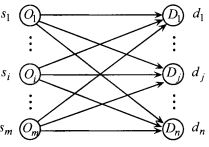
\includegraphics[scale=1.2]{transporte}
\end{center}


El problema es determinar qué cantidades hay que trasladar desde $i$ hasta $j$ de forma que se minimice el coste total del transporte.

\end{frame}
%----------------------------------------------
\begin{frame}
\frametitle{Problema de asignación}


\begin{center}
\textit{Cada trabajo para el mejor trabajador posible}
\end{center}


\

Hay que asignar $n$ tareas a $n$ trabajadores. Si se asigna la tarea $i$ al trabajador $j$ se incurre en un coste de $c_{ij}$.


\

El problema es asignar las tareas a los trabajadores de manera que se minimice el coste.




\end{frame}


%----------------------------------------------
\begin{frame}
\frametitle{Flujo de coste mínimo en una red}


Se considera una red con $n$ nodos $i=1,\ldots,n$.

\

En cada nodo hay una oferta $b_i>0$ (demanda si $b_i<0$).

\

La red está equilibrada: $\sum_{i=1}^n b_i=0$.

\

Asociado a cada arco $(i,j)$ hay un coste unitario de flujo $c_{ij}$.

\

Problema: determinar el flujo $x_{ij}\geq 0$ de coste mínimo tal  que el flujo neto (cantidad de salida menos cantidad de llegada) en cada nodo sea $b_i$. 


\end{frame}
%----------------------------------------------
\begin{frame}
\frametitle{Flujo de coste mínimo en una red}

El grafo representa una red ferroviaria de seis ciudades.
Hay dos locomotoras en el nodo 2 y una más en el nodo 1. Se requieren tres locomotoras en el 6. En cada arco aparece el coste de trasladar una locomotora entre cada dos nodos. 

\begin{center}
\includegraphics[height=5cm]{grafo.pdf}
\end{center}

Plantear el problema de cómo trasladar las locomotoras con el mínimo coste.

\end{frame}
%----------------------------------------------
\begin{frame}
\frametitle{Forma estándar de un problema lineal}

Un problema lineal siempre se puede escribir en la siguiente \textbf{forma estándar}:
\begin{center}
\begin{tabular}{ll}
minimizar & $c_1x_1 +\cdots +  c_nx_n$ \\
s.a. & $a_{11}x_1+\cdots + a_{1n}x_n = b_1$    \\
	& $\cdots$	\\
	& $a_{m1}x_1+\cdots + a_{mn}x_n = b_m$    \\
	 & $x_1\geq 0,\ \cdots, x_n\geq 0$
\end{tabular}
\end{center}

\

Matricialmente:

\begin{center}
\begin{tabular}{lr}
minimizar & $c^\top x$ \\
s.a. & $Ax=b$   \\
	 & $x\geq 0$
\end{tabular}
\end{center}

\end{frame}
%----------------------------------------------
\begin{frame}
\frametitle{Para escribir un problema en forma estándar}



\begin{itemize}

\item Maximizar una función $f$ equivale a minimizar $-f$.

\item Si una restricción es   
\[
a_{j1}x_1+\cdots + a_{jn}x_n \leq b_j,
\] se añade una \textbf{variable de holgura} $x_{n+1}\geq 0$ para obtener 
\[
a_{j1}x_1+\cdots + a_{jn}x_n + x_{n+1} = b_j.
\]

\item Si una restricción es   
\[
a_{j1}x_1+\cdots + a_{jn}x_n \geq b_j,
\]
se multiplica por $-1$ y se aplica el punto anterior.

\item Si una variable $x_i$ no está restringida a tomar valores positivos se expresa como diferencia de dos variables positivas:
\[
x_i = x'_i-x''_i, \ \ x'_i\geq 0, \ x''_i\geq 0.
\]

\end{itemize}




\end{frame}
\begin{frame}
\frametitle{Escribe en forma estándar}



\begin{tabular}{lr}
maximizar & $3x_1 + 2x_3$ \\
s.a. & $x_1+ x_2 + x_3 \leq 1$    \\
	& $x_1 - x_2 \geq 5$ \\
	 & $x_1\geq 0,\ x_2\geq 0, x_3\geq 0$
\end{tabular}


\

\


\begin{tabular}{lr}
minimizar & $2x_1 + x_2$ \\
s.a. & $x_1 - 2x_2 = 0$    \\
	 & $x_2\geq 1$
\end{tabular}

\

\

\begin{tabular}{lr}
maximizar & $x_1 + 4x_2+x_3$ \\
s.a. & $2x_1 - 2x_2 + x_3 = 4$    \\
	& $x_1 - x_3 = 1$ \\
	 & $x_2\geq 0, x_3\geq 0$
\end{tabular}


\end{frame}
%----------------------------------------------
\begin{frame}
\frametitle{Forma canónica de un problema lineal}

Un problema lineal siempre se puede escribir en la siguiente \textbf{forma canónica}:

\

Problemas de minimización:


\begin{center}
\begin{tabular}{lr}
minimizar & $c^\top x$ \\
s.a. & $Ax \geq b$   \\
	 & $x\geq 0$
\end{tabular}
\end{center}


\
 
Problemas de maximización:


\begin{center}
\begin{tabular}{lr}
maximizar & $c^\top x$ \\
s.a. & $Ax \leq b$   \\
	 & $x\geq 0$
\end{tabular}
\end{center}

\end{frame}

%----------------------------------------------
\begin{frame}
\frametitle{Problemas de optimización convexos}


Son problemas de minimización en los que la función objetivo es convexa, las funciones que definen las restricciones de desigualdad también son convexas y las restricciones de igualdad son lineales. 

\

Formalmente,
\begin{center}
\begin{tabular}{lll}
minimizar & $f(x)$ & \\
s.a. & $f_i(x)\leq 0,$  &  $i=1,\ldots,m$ \\
	 & $a^\top_i x = b_i,$  &  $i=1,\ldots,p$,
\end{tabular}
\end{center}
donde las funciones $f,f_1,\ldots, f_n$ son convexas.

\


Si el problema es de maximización, para que el problema sea convexo la función objetivo debe ser cóncava.

\end{frame}
%----------------------------------------------
\begin{frame}
\frametitle{Ejemplo: optimización de una cartera de acciones}

Un inversor quiere decidir qué proporción  $x_i$ de los fondos disponibles invierte
en $n$ posibles acciones cuyos beneficios $r_i$, con $i=1,\ldots,n$, son variables aleatorias tales que $\mathbb{E}(r_i)=\mu_i$, $\mbox{Var}(r_i)=\sigma^2_i$ y 
\[
\mbox{Cov}(r_i,r_j) = \sigma_{ij} = \mathbb{E}[(r_i-\mu_i)(r_j-\mu_j)], \ \ i,j=1,\ldots, n.
\]
El beneficio obtenido es $R=\sum_{i=1}^n x_ir_i$.


\

\textbf{Beneficio esperado:} 
\[
\mathbb{E}(R)=\sum_{i=1}^n x_i\mu_i := x^\top \mu.
\]

\

\textbf{Varianza (riesgo) del beneficio:}
\[
\mbox{Var}(R) = \sum_{i=1}^n \sum_{j=1}^n x_ix_j\sigma_{ij} = x^\top\Sigma x.
\]
  
\end{frame}
%----------------------------------------------
\begin{frame}
\frametitle{Ejemplo: optimización de una cartera de acciones}

El objetivo general es maximizar el beneficio con el menor riesgo posible.

\

Un posible problema a resolver para encontrar la cartera óptima:
\begin{center}
\begin{tabular}{lr}
maximizar & $x^\top\mu - \lambda x^\top\Sigma x$ \\
s.a. & $\sum_{i=1}^n x_i=1$    \\
	& $x\geq 0$,
\end{tabular}
\end{center}
donde $\lambda>0$ es un parámetro que refleja la aversión al riesgo.

\

Como $\Sigma$ es semidefinida positiva, puede demostrarse que la función objetivo es cóncava, mientras que las restricciones son lineales. Se trata de un \textbf{problema de optimización convexo} (cuadrático).


\end{frame}
%----------------------------------------------------------------------
\end{document}
%----------------------------------------------------------------------


%----------------------------------------------
\begin{frame}
\frametitle{}

\end{frame}
%--------------------------------------------